% Generated by Sphinx.
\def\sphinxdocclass{report}
\documentclass[a4paper,10pt,english]{sphinxmanual}
\usepackage[utf8]{inputenc}
\DeclareUnicodeCharacter{00A0}{\nobreakspace}
\usepackage[T1]{fontenc}
\usepackage{babel}
\usepackage{times}
\usepackage[Bjarne]{fncychap}
\usepackage{longtable}
\usepackage{sphinx}
\usepackage{multirow}


\title{Personis Documentation}
\date{July 31, 2012}
\release{12.9}
\author{Bob Kummerfeld and Judy Kay}
\newcommand{\sphinxlogo}{}
\renewcommand{\releasename}{Release}
\makeindex

\makeatletter
\def\PYG@reset{\let\PYG@it=\relax \let\PYG@bf=\relax%
    \let\PYG@ul=\relax \let\PYG@tc=\relax%
    \let\PYG@bc=\relax \let\PYG@ff=\relax}
\def\PYG@tok#1{\csname PYG@tok@#1\endcsname}
\def\PYG@toks#1+{\ifx\relax#1\empty\else%
    \PYG@tok{#1}\expandafter\PYG@toks\fi}
\def\PYG@do#1{\PYG@bc{\PYG@tc{\PYG@ul{%
    \PYG@it{\PYG@bf{\PYG@ff{#1}}}}}}}
\def\PYG#1#2{\PYG@reset\PYG@toks#1+\relax+\PYG@do{#2}}

\def\PYG@tok@gd{\def\PYG@tc##1{\textcolor[rgb]{0.63,0.00,0.00}{##1}}}
\def\PYG@tok@gu{\let\PYG@bf=\textbf\def\PYG@tc##1{\textcolor[rgb]{0.50,0.00,0.50}{##1}}}
\def\PYG@tok@gt{\def\PYG@tc##1{\textcolor[rgb]{0.00,0.25,0.82}{##1}}}
\def\PYG@tok@gs{\let\PYG@bf=\textbf}
\def\PYG@tok@gr{\def\PYG@tc##1{\textcolor[rgb]{1.00,0.00,0.00}{##1}}}
\def\PYG@tok@cm{\let\PYG@it=\textit\def\PYG@tc##1{\textcolor[rgb]{0.25,0.50,0.56}{##1}}}
\def\PYG@tok@vg{\def\PYG@tc##1{\textcolor[rgb]{0.73,0.38,0.84}{##1}}}
\def\PYG@tok@m{\def\PYG@tc##1{\textcolor[rgb]{0.13,0.50,0.31}{##1}}}
\def\PYG@tok@mh{\def\PYG@tc##1{\textcolor[rgb]{0.13,0.50,0.31}{##1}}}
\def\PYG@tok@cs{\def\PYG@tc##1{\textcolor[rgb]{0.25,0.50,0.56}{##1}}\def\PYG@bc##1{\colorbox[rgb]{1.00,0.94,0.94}{##1}}}
\def\PYG@tok@ge{\let\PYG@it=\textit}
\def\PYG@tok@vc{\def\PYG@tc##1{\textcolor[rgb]{0.73,0.38,0.84}{##1}}}
\def\PYG@tok@il{\def\PYG@tc##1{\textcolor[rgb]{0.13,0.50,0.31}{##1}}}
\def\PYG@tok@go{\def\PYG@tc##1{\textcolor[rgb]{0.19,0.19,0.19}{##1}}}
\def\PYG@tok@cp{\def\PYG@tc##1{\textcolor[rgb]{0.00,0.44,0.13}{##1}}}
\def\PYG@tok@gi{\def\PYG@tc##1{\textcolor[rgb]{0.00,0.63,0.00}{##1}}}
\def\PYG@tok@gh{\let\PYG@bf=\textbf\def\PYG@tc##1{\textcolor[rgb]{0.00,0.00,0.50}{##1}}}
\def\PYG@tok@ni{\let\PYG@bf=\textbf\def\PYG@tc##1{\textcolor[rgb]{0.84,0.33,0.22}{##1}}}
\def\PYG@tok@nl{\let\PYG@bf=\textbf\def\PYG@tc##1{\textcolor[rgb]{0.00,0.13,0.44}{##1}}}
\def\PYG@tok@nn{\let\PYG@bf=\textbf\def\PYG@tc##1{\textcolor[rgb]{0.05,0.52,0.71}{##1}}}
\def\PYG@tok@no{\def\PYG@tc##1{\textcolor[rgb]{0.38,0.68,0.84}{##1}}}
\def\PYG@tok@na{\def\PYG@tc##1{\textcolor[rgb]{0.25,0.44,0.63}{##1}}}
\def\PYG@tok@nb{\def\PYG@tc##1{\textcolor[rgb]{0.00,0.44,0.13}{##1}}}
\def\PYG@tok@nc{\let\PYG@bf=\textbf\def\PYG@tc##1{\textcolor[rgb]{0.05,0.52,0.71}{##1}}}
\def\PYG@tok@nd{\let\PYG@bf=\textbf\def\PYG@tc##1{\textcolor[rgb]{0.33,0.33,0.33}{##1}}}
\def\PYG@tok@ne{\def\PYG@tc##1{\textcolor[rgb]{0.00,0.44,0.13}{##1}}}
\def\PYG@tok@nf{\def\PYG@tc##1{\textcolor[rgb]{0.02,0.16,0.49}{##1}}}
\def\PYG@tok@si{\let\PYG@it=\textit\def\PYG@tc##1{\textcolor[rgb]{0.44,0.63,0.82}{##1}}}
\def\PYG@tok@s2{\def\PYG@tc##1{\textcolor[rgb]{0.25,0.44,0.63}{##1}}}
\def\PYG@tok@vi{\def\PYG@tc##1{\textcolor[rgb]{0.73,0.38,0.84}{##1}}}
\def\PYG@tok@nt{\let\PYG@bf=\textbf\def\PYG@tc##1{\textcolor[rgb]{0.02,0.16,0.45}{##1}}}
\def\PYG@tok@nv{\def\PYG@tc##1{\textcolor[rgb]{0.73,0.38,0.84}{##1}}}
\def\PYG@tok@s1{\def\PYG@tc##1{\textcolor[rgb]{0.25,0.44,0.63}{##1}}}
\def\PYG@tok@gp{\let\PYG@bf=\textbf\def\PYG@tc##1{\textcolor[rgb]{0.78,0.36,0.04}{##1}}}
\def\PYG@tok@sh{\def\PYG@tc##1{\textcolor[rgb]{0.25,0.44,0.63}{##1}}}
\def\PYG@tok@ow{\let\PYG@bf=\textbf\def\PYG@tc##1{\textcolor[rgb]{0.00,0.44,0.13}{##1}}}
\def\PYG@tok@sx{\def\PYG@tc##1{\textcolor[rgb]{0.78,0.36,0.04}{##1}}}
\def\PYG@tok@bp{\def\PYG@tc##1{\textcolor[rgb]{0.00,0.44,0.13}{##1}}}
\def\PYG@tok@c1{\let\PYG@it=\textit\def\PYG@tc##1{\textcolor[rgb]{0.25,0.50,0.56}{##1}}}
\def\PYG@tok@kc{\let\PYG@bf=\textbf\def\PYG@tc##1{\textcolor[rgb]{0.00,0.44,0.13}{##1}}}
\def\PYG@tok@c{\let\PYG@it=\textit\def\PYG@tc##1{\textcolor[rgb]{0.25,0.50,0.56}{##1}}}
\def\PYG@tok@mf{\def\PYG@tc##1{\textcolor[rgb]{0.13,0.50,0.31}{##1}}}
\def\PYG@tok@err{\def\PYG@bc##1{\fcolorbox[rgb]{1.00,0.00,0.00}{1,1,1}{##1}}}
\def\PYG@tok@kd{\let\PYG@bf=\textbf\def\PYG@tc##1{\textcolor[rgb]{0.00,0.44,0.13}{##1}}}
\def\PYG@tok@ss{\def\PYG@tc##1{\textcolor[rgb]{0.32,0.47,0.09}{##1}}}
\def\PYG@tok@sr{\def\PYG@tc##1{\textcolor[rgb]{0.14,0.33,0.53}{##1}}}
\def\PYG@tok@mo{\def\PYG@tc##1{\textcolor[rgb]{0.13,0.50,0.31}{##1}}}
\def\PYG@tok@mi{\def\PYG@tc##1{\textcolor[rgb]{0.13,0.50,0.31}{##1}}}
\def\PYG@tok@kn{\let\PYG@bf=\textbf\def\PYG@tc##1{\textcolor[rgb]{0.00,0.44,0.13}{##1}}}
\def\PYG@tok@o{\def\PYG@tc##1{\textcolor[rgb]{0.40,0.40,0.40}{##1}}}
\def\PYG@tok@kr{\let\PYG@bf=\textbf\def\PYG@tc##1{\textcolor[rgb]{0.00,0.44,0.13}{##1}}}
\def\PYG@tok@s{\def\PYG@tc##1{\textcolor[rgb]{0.25,0.44,0.63}{##1}}}
\def\PYG@tok@kp{\def\PYG@tc##1{\textcolor[rgb]{0.00,0.44,0.13}{##1}}}
\def\PYG@tok@w{\def\PYG@tc##1{\textcolor[rgb]{0.73,0.73,0.73}{##1}}}
\def\PYG@tok@kt{\def\PYG@tc##1{\textcolor[rgb]{0.56,0.13,0.00}{##1}}}
\def\PYG@tok@sc{\def\PYG@tc##1{\textcolor[rgb]{0.25,0.44,0.63}{##1}}}
\def\PYG@tok@sb{\def\PYG@tc##1{\textcolor[rgb]{0.25,0.44,0.63}{##1}}}
\def\PYG@tok@k{\let\PYG@bf=\textbf\def\PYG@tc##1{\textcolor[rgb]{0.00,0.44,0.13}{##1}}}
\def\PYG@tok@se{\let\PYG@bf=\textbf\def\PYG@tc##1{\textcolor[rgb]{0.25,0.44,0.63}{##1}}}
\def\PYG@tok@sd{\let\PYG@it=\textit\def\PYG@tc##1{\textcolor[rgb]{0.25,0.44,0.63}{##1}}}

\def\PYGZbs{\char`\\}
\def\PYGZus{\char`\_}
\def\PYGZob{\char`\{}
\def\PYGZcb{\char`\}}
\def\PYGZca{\char`\^}
\def\PYGZsh{\char`\#}
\def\PYGZpc{\char`\%}
\def\PYGZdl{\char`\$}
\def\PYGZti{\char`\~}
% for compatibility with earlier versions
\def\PYGZat{@}
\def\PYGZlb{[}
\def\PYGZrb{]}
\makeatother

\begin{document}

\maketitle
\tableofcontents
\phantomsection\label{index::doc}


Contents:


\chapter{Introduction}
\label{Intro:introduction}\label{Intro::doc}\label{Intro:personis-user-modeling-framework}\begin{itemize}
\item {} 
User Models as first class citizens
\begin{itemize}
\item {} 
independant of a particular application

\item {} 
not just fragments of me locked away in individual systems

\item {} 
may be distributed over machines I use or in the cloud (could be a personal cloud)

\end{itemize}

\item {} 
Scutability and user control
\begin{itemize}
\item {} 
I own my model

\item {} 
I control what goes in

\item {} 
I control what goes out (releasing parts to applications)

\item {} 
I can see my model in meaningful forms

\end{itemize}

\item {} 
as new evidence about an aspect is available an application (evidence source) \emph{tells} the user model

\item {} 
the user model \emph{accretes} the evidence
\begin{itemize}
\item {} 
a times stamp is added

\item {} 
the source (registered name of the application) is added

\item {} 
the evidence type (explicit,...) is added

\item {} 
the evidence is appended to a list associated with a component of the model

\end{itemize}

\end{itemize}

Resolution:
\begin{itemize}
\item {} 
When an application needs to know information from the model, it asks the model for the value of the required set of components, it \emph{asks} the model for the required set of components

\item {} 
At that time
\begin{itemize}
\item {} 
A filter selects the evidence allowed to the asker

\item {} 
A resolver function interprets the allowed evidence
\begin{itemize}
\item {} 
the application may specify the resolver function (from those allowed)

\item {} 
Or use default

\item {} 
Can be very simple (eg Point Query) or arbitrarily sophisticated (eg use Bayesian model, ontology.)

\end{itemize}

\end{itemize}

\item {} 
Embrace inconsistency, multiple interpretations!

\end{itemize}

Scrutability:
\begin{description}
\item[{Definition:}] \leavevmode\begin{quote}

Capable of being understood through study and observation, comprehensible.
(www.thefreedictionary.com/scrutable)

Understandable upon close examination. (www.tiscali.co.uk/reference/dictionaries/difficultwords/data/d0011288.html)
\end{quote}
\begin{itemize}
\item {} 
the Personis Framework is designed for scrutability
\begin{itemize}
\item {} 
Why did the system adapt that way?

\item {} 
Where does the system think I am, and why?

\item {} 
Historic queries: what location did the system think I was on May 1st 2001?

\item {} 
what music does the system think I like and why?

\end{itemize}

\end{itemize}

\end{description}

Model Structure:
\begin{itemize}
\item {} 
the model is represented as a tree

\item {} 
we call the branches \emph{contexts} and the leaves \emph{components}

\end{itemize}

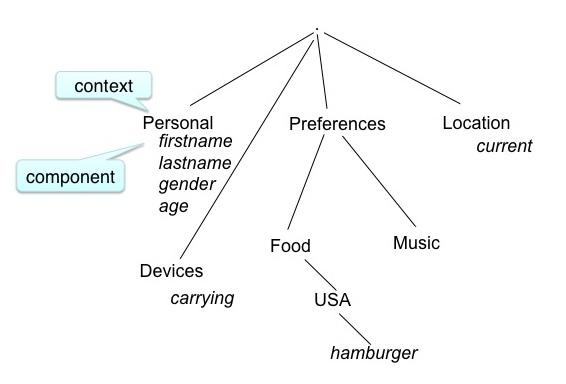
\includegraphics{model-tree.jpg}

Atomic modelled unit - component:

The components of a model contain the evidence associated with that attribute. Example components:
\begin{itemize}
\item {} 
for classic user model:
\begin{itemize}
\item {} 
knowledge

\item {} 
beliefs

\item {} 
preferences

\end{itemize}

\item {} 
for pervasive computing:
\begin{itemize}
\item {} 
attributes (eg weight, location, sensor reading)

\item {} 
qualifiers for knowledge and attributes

\item {} 
goals (eg I want to be able to do 10 chin-ups)

\end{itemize}

\end{itemize}
\begin{description}
\item[{Operation:}] \leavevmode\begin{quote}

tell
\end{quote}
\begin{itemize}
\item {} 
evidence is accreted by components after the \emph{tell} operation

\end{itemize}

\end{description}

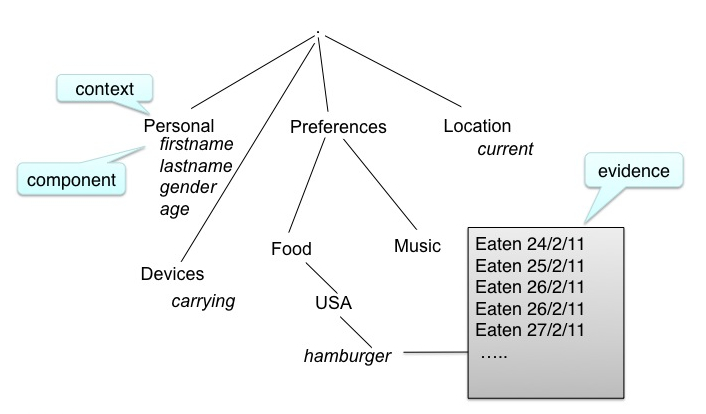
\includegraphics{accretion.jpg}
\begin{description}
\item[{Operation:}] \leavevmode\begin{quote}

ask
\end{quote}
\begin{itemize}
\item {} 
A component value is retrieved from the nodel using an \emph{ask} operation
\begin{itemize}
\item {} 
the evidence is \emph{resolved} by a resolver function to give the value

\end{itemize}

\end{itemize}

\end{description}

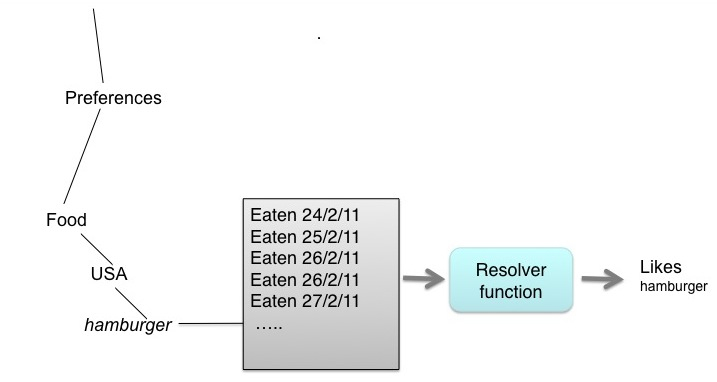
\includegraphics{resolution.jpg}

Accretion/Resolution
\begin{itemize}
\item {} 
values are only calculated from the evidence when they are needed, rather than whenever a new data point (evidence) is received

\item {} 
the choice of resolver function allows flexibility in the calculated values. For example, location may be resolved as:
\begin{itemize}
\item {} 
room 123, or ``at work'', or latitude/longitude

\end{itemize}

\item {} 
historic queries are possible: where was I on a certain date, how have my music preferences changed.

\end{itemize}


\chapter{Documentation}
\label{Documentation:documentation}\label{Documentation::doc}
The documentation for Personis is built using the \emph{sphinx}, a python based documentation generation tool.
Sphinx can make the documentation in many forms.
To use the tool you need to install sphinx and its dependancies.
A generated pdf version is included in the distribution.
If you want to make the pdf version you will need to install a full latex package (eg texlive-full).

To make the various versions the command is:

\begin{DUlineblock}{0em}
\item[] make html
\item[] make latexpdf
\item[] make epub
\end{DUlineblock}

The generated versions are placed in the subdirectory ``\_build''.


\chapter{Installation}
\label{Installation:installation}\label{Installation::doc}
These installation instructions assume that you are installing Personis on a linux system with Python 2.6 or 2.7
installed.

The Personis framework makes use of several packages that are not part
of the default Python installation.
The packages are:
\begin{itemize}
\item {} 
cherrypy (version 3.x)

\item {} 
pyparsing

\item {} 
google oauth2

\item {} 
httplib2

\end{itemize}

Personis is known to work with these versions and copies are included in
the Personis distribution for your convenience. Personis may work with
more recent versions but this has not been tested.

Quick installation instructions:

The distribution of personis is a compressed tar file: Personis-rrr.tgz

First untar the distribution (\emph{rrr} is the release number):

\begin{Verbatim}[commandchars=\\\{\}]
\$ tar zxf Personis-rrr.tgz
\end{Verbatim}

This will create a directory Personis-rrr for the code:

\begin{Verbatim}[commandchars=\\\{\}]
\$ cd Personis-rrr
\$ ls
Apps            Personis        README          install.sh
\end{Verbatim}

To install Personis, use the command:

\begin{Verbatim}[commandchars=\\\{\}]
\$ ./install.sh
\end{Verbatim}

The Personis modules are in the Personis/Src directory and can be run directly
from that directory or any other directory by setting your PYTHONPATH
environment variable.
Necessary support packages will be installed in the Personis/lib/python
directory and so that directory must also be in the PYTHONPATH.

The following commands will set the path (where \emph{rrr} is the release number):

\begin{Verbatim}[commandchars=\\\{\}]
cd Personis-rrr
export PYTHONPATH={}`pwd{}`/Personis/Src:{}`pwd{}`/Personis/lib/python
\end{Verbatim}

You might want to note the value of PYTHONPATH and add a line to
your .bashrc to set it for future use.


\chapter{Tests}
\label{Tests:tests}\label{Tests::doc}
The test scripts are divided into those that test the base Personis
module for models stored on the local machine (base), and those that
test the server Personis module for models accessed via a network
connection (server). In both cases the driver test script gives you the
option of nominating a directory to store test models. In the base case
the models are accessed directly by the methods in the Personis\_base
module. In the server case, a Personis server is started to provide
access to the models.

To run the tests, change into the Personis directory and:

\begin{Verbatim}[commandchars=\\\{\}]
\$ bash Tests/base-tests
PYTHONPATH is ....../Personis/Src
model directory? [..../Tests/Models]
\end{Verbatim}

at this point the test script is asking for a directory to store the test models. The default directory
is ``Models'' in the Tests directory. You can accept this default by pressing return, or type another pathname.

You are now given the option of removing any models previously placed in the test directory. This is useful if
you want to rerun the tests from scratch and create the models again. If you press return you will get
the default response of ``No'', typing ``Y'' will remove the existing models:

\begin{Verbatim}[commandchars=\\\{\}]
Remove models in ......./Src/models? [N]
\end{Verbatim}

If you say Yes (or when you run it for the first time) the models will be recreated.
This will produce a lot of output showing all the model parts as they are created.

Next you are given the option of running all the available base tests, running a particular test, or no tests.
The base test scripts are stored in the directory Tests/Base and are numbered. If you are testing a particular
feature you can type the number, but to start we suggest typing return for all tests.
The tests now run, one a time, waiting for you to press return before starting the next. If you want to stop
you can press Control-C:

\begin{Verbatim}[commandchars=\\\{\}]
Test number? (CR for all, ctrl-C if none)

Running tests...

====================================================================
                          Tests/Base/example01\_add.py
====================================================================
add evidence to alice's model
===================================================================
Now check the evidence list for alice's names
===================================================================
Component:  First name
===================================================================


        ...lots more output...


=================
All Done.
=================
\end{Verbatim}

There should be only a small number of python error messages and these will have some explanation in the output.

There are a set of similar tests for the server that can be run with the command:

\begin{Verbatim}[commandchars=\\\{\}]
\$ bash Tests/server-tests

        ...lots of output...

=================
All Done.
=================
\end{Verbatim}

The models are created in a similar way for the server tests but a server process is started and the
client-server protocol used to access them. The server test scripts can be found in Tests/Server.


\chapter{Tutorial Introduction to Personis}
\label{Tutorial::doc}\label{Tutorial:tutorial-introduction-to-personis}
This tutorial assumes you have installed the framework using the instructions in the Installation section.
Using the \emph{umbrowser} command line utility, the tutorial will take you through the construction, navigation and
management of a user model.


\section{umbrowser}
\label{Tutorial:umbrowser}
The umbrowser.py program is a commandline utility that allows most
operations of the Personis system to be carried out interactively.

Umbrowser is found in the main Personis directory and is started with
the command ./umbrowser.py:

\begin{Verbatim}[commandchars=\\\{\}]
\$ ./umbrowser.py
[''] \textgreater{}
\end{Verbatim}

The prompt indicates that the browser is waiting for a command. The
initial part shows the current context, with the root context as an
empty string.

The help command gives information about the available commands:

\begin{Verbatim}[commandchars=\\\{\}]
[''] \textgreater{} help
Documented commands (type help \textless{}topic\textgreater{}):
========================================
app         delapp        export      login        mkmodel  set       subscribe
attributes  delcomponent  import      ls           model    setgoals  tell
base        delsub        importmdef  mkcomponent  quit     setperm
cd          do            listapps    mkcontext    server   showperm

Undocumented commands:
======================
help
\end{Verbatim}

To create or access a model you need to specify a username and password
using the login command:

\begin{Verbatim}[commandchars=\\\{\}]
[''] \textgreater{} help login
login username password
[''] \textgreater{} login alice secret
username: alice
password: secret
\end{Verbatim}

To operate on models stored in the local file system we use the ``base''
command. To operate on models stored on a remote server we user the
``server'' command. For now we will use ``base'' since we can only make new models in the local file system,
not remotely:

\begin{Verbatim}[commandchars=\\\{\}]
\PYG{p}{[}\PYG{l+s}{'}\PYG{l+s}{'}\PYG{p}{]} \PYG{o}{\textgreater{}} \PYG{n}{base}
\end{Verbatim}

Now we make a model for alice in the current directory (.) using the
mkmodel command:

\begin{Verbatim}[commandchars=\\\{\}]
[''] \textgreater{} help mkmodel
 mkmodel model\_name [model\_directory]
        makes a new empty model
        uses username, password specified in login cmd

[''] \textgreater{} mkmodel Alice .

making model 'Alice' in directory '.' with username 'alice' and password 'secret'
model made
to access the model, use the command 'model Alice .'
\end{Verbatim}

Note that we called the model ``Alice''. This could be the same as the login
name but that is not necessary. For example user alice might want to make a
model for a temperature sensing device and might call the model ``Temp''.
Model names are case sensitive, so ``Alice'' is not the same as ``alice''.

Also, we could have put the model anywhere in the file system but chose
to put it in the current directory (.). The model is actually store in a
directory with the same name as the model. So, after the mkmodel command
there will be a new directory called ``Alice'' in our current directory.

Now we want to access the new model, so we use the ``model'' command:

\begin{Verbatim}[commandchars=\\\{\}]
 [''] \textgreater{} model Alice .
model 'Alice' open, access type is 'base'
\end{Verbatim}

and now we can see what is in the model (should be empty):

\begin{Verbatim}[commandchars=\\\{\}]
Alice [''] \textgreater{} ls
Components:
Contexts: []
Views: \PYGZob{}\PYGZcb{}
Subscriptions: \PYGZob{}\PYGZcb{}
\end{Verbatim}

The ``ls'' command is a like the Unix ls command: it lists what is in the
current context.
As you can see, the model is empty - no components, contexts, views or
subscriptions.
So let's make a new context called ``Prefs'' in the current (root) context:

\begin{Verbatim}[commandchars=\\\{\}]
Alice [''] \textgreater{} mkcontext Prefs
Context description? My preferences
Create new context 'Prefs' in context '['']' with description 'My preferences'
Ok?[N] Y

Alice [''] \textgreater{} ls
Components:
Contexts: ['Prefs']
Views: \PYGZob{}\PYGZcb{}
Subscriptions: \PYGZob{}\PYGZcb{}
\end{Verbatim}

Now we will change context to the new ``Prefs'' context and make a
component ``food'' for our food preferences:

\begin{Verbatim}[commandchars=\\\{\}]
Alice [''] \textgreater{} cd Prefs

Alice ['', 'Prefs'] \textgreater{} mkcomponent food
Component description? type of food I prefer
Component type:
0 attribute
1 activity
2 knowledge
3 belief
4 preference
5 goal
Index? 4
Value type:
0 string
1 number
2 boolean
3 enum
4 JSON
Index? 0
Creating new component 'food', type 'preference', description 'type of food I prefer', value type 'string'
Ok?[N] Y

Alice ['', 'Prefs'] \textgreater{} ls
Components:
        food: type of food I prefer
Contexts: []
Views: \PYGZob{}\PYGZcb{}
Subscriptions: \PYGZob{}\PYGZcb{}

Alice ['', 'Prefs'] \textgreater{}
\end{Verbatim}

Now we have a model called ``Alice'', owned by ``alice'' that has one
context ``Prefs'' containing one component ``food''.
Now, Alice likes Thai food so we will add some evidence to her food
preference component using the ``tell'' command:

\begin{Verbatim}[commandchars=\\\{\}]
Alice ['', 'Prefs'] \textgreater{} tell food
Value? Thai
Evidence type:
0 explicit
1 implicit
2 exmachina
3 inferred
4 stereotype
Index? [0]
Evidence flag? (CR for none)
Tell value=Thai, type=explicit, flags=[], source=alice, context=['', 'Prefs'], component=food
Ok?[N] Y


Alice ['', 'Prefs'] \textgreater{} ls
Components:
        food: type of food I prefer
Contexts: []
Views: \PYGZob{}\PYGZcb{}
Subscriptions: \PYGZob{}\PYGZcb{}
\end{Verbatim}

We can now examine the ``food'' component with the ``ls'' command:

\begin{Verbatim}[commandchars=\\\{\}]
Alice ['', 'Prefs'] \textgreater{} ls food
===================================================================
Component:  type of food I prefer
===================================================================
showobj:
  Description = type of food I prefer
  component\_type = preference
  evidencelist = 1 items
  value\_list = []
  value = Thai
  value\_type = string
  goals = []
  resolver = None
  Identifier = food
  objectType = Component
---------------------------------
Evidence about it
---------------------------------
showobj:
           comment = None
           evidence\_type = explicit
           value = Thai
           objectType = Evidence
           source = alice
           flags = ['']
           time = Thu Apr 28 18:08:55 2011 (1304003335.61)
           owner = alice
           exp\_time = 0
           useby = None
---------------------------------
\end{Verbatim}

Try doing the ``tell'' operation again with a different food preference and then ``ls food'' to see the additional
evidence that has been accreted.

To quit the model browser, use the \emph{quit} command.


\chapter{Personis Server}
\label{Server::doc}\label{Server:personis-server}
Personis operates as a library that is imported by application programs and stores models in the local file
system.

Personis can also be run as a server, providing an interface to models for remote clients. In this case the API is almost the same, the only difference being the modules that is imported and used for the Access call, and the
specification of the model to be accessed.

In the case of locally stored models, access requires a \emph{modeldir} argument to specify the
location of the stored models, as well as the name of the model (a simple ID).
For models accessed remotely via the server, \emph{modeldir} is not used and the model name has the form:
name@server{[}:port{]}.

For example, to access the model for ``alice'' stored on the server ``models.server.com'' we
would use the statements:

\begin{Verbatim}[commandchars=\\\{\}]
\PYG{k+kn}{import} \PYG{n+nn}{Personis}

\PYG{n}{um} \PYG{o}{=} \PYG{n}{Personis}\PYG{o}{.}\PYG{n}{Access}\PYG{p}{(}\PYG{n}{model}\PYG{o}{=}\PYG{l+s}{"}\PYG{l+s}{alice@models.server.com}\PYG{l+s}{"}\PYG{p}{,} \PYG{n}{user}\PYG{o}{=}\PYG{l+s}{'}\PYG{l+s}{myapp}\PYG{l+s}{'}\PYG{p}{,} \PYG{n}{password}\PYG{o}{=}\PYG{l+s}{'}\PYG{l+s}{pass}\PYG{l+s}{'}\PYG{p}{)}
\end{Verbatim}


\section{Running a Server}
\label{Server:running-a-server}
It is very easy to run your own Personis server to provide access to models for remote clients.

A server gets configuration information from the file \$HOME/.personis\_server.conf.
This file specifies the port that the server is to use as well as some miscellaneous configuration options.
A suitable personis\_server.conf file can be found in the Personis/Src directory. This can be copied into
\$HOME/.personis\_server.conf and the port number changed as desired.

A server can be started for any set of models stored in the same directory using the command:

\begin{Verbatim}[commandchars=\\\{\}]
\# assuming that PYTHONPATH, MODELDIR and LOGFILE are initialised
Personis.py  --models \$MODELDIR --log \$LOGFILE \&
\end{Verbatim}

The directory containing the models is specified in \$MODELDIR.
Log information is written to \$LOGFILE. This includes information on all requests, error messages etc.


\chapter{Example Applications}
\label{Examples::doc}\label{Examples:example-applications}

\section{Museum Guide}
\label{Examples:museum-guide}

\section{Health Monitoring}
\label{Examples:health-monitoring}

\section{Drill and Practice}
\label{Examples:drill-and-practice}

\chapter{Application Program Interface}
\label{API:application-program-interface}\label{API::doc}
\textbf{Files}

\begin{tabulary}{\linewidth}{|L|L|}
\hline
\textbf{
File
} & \textbf{
Description
}\\\hline

Personis\_base.py
 & 
the core library that accesses models in local directories/files
\\\hline

Personis\_a.py
 & 
adds `Active User Models' to Personis. This allows components to
be `subscribable' and statements in a simple language to be executed
when new component values satisfy a condition.
\\\hline

Personis\_base.py
 & 
the core library that accesses models in local directories/files
\\\hline

Personis\_a.py
 & 
adds `Active User Models' to Personis. This allows components to
be `subscribable' and statements in a simple language to be executed
when new component values satisfy a condition.
\\\hline

Personis\_server.py
 & 
a server and set of stubs for the server version of Personis
uses Personis\_a.py to do the work
\\\hline

Personis.py
 & 
a wrapper for Personis\_server
\\\hline

Tests/*
 & 
scripts to test the system
\\\hline

Tests/Base/example*
 & 
a set of code examples for models stored locally
\\\hline

Tests/Server/example*
 & 
a set of code examples for models stored on a server
\\\hline

mkmodel
 & 
utility program to make a set of models from a
\\\hline

modeldef
 & 
definition file
\\\hline
\end{tabulary}


\textbf{Constants}

ComponentTypes:

\begin{Verbatim}[commandchars=\\\{\}]
\PYG{l+s}{"}\PYG{l+s}{attribute}\PYG{l+s}{"}
\PYG{l+s}{"}\PYG{l+s}{activity}\PYG{l+s}{"}
\PYG{l+s}{"}\PYG{l+s}{knowledge}\PYG{l+s}{"}
\PYG{l+s}{"}\PYG{l+s}{belief}\PYG{l+s}{"}
\PYG{l+s}{"}\PYG{l+s}{preference}\PYG{l+s}{"}
\PYG{l+s}{"}\PYG{l+s}{goal}\PYG{l+s}{"}
\end{Verbatim}

ValueTypes:

\begin{Verbatim}[commandchars=\\\{\}]
\PYG{l+s}{"}\PYG{l+s}{string}\PYG{l+s}{"}
\PYG{l+s}{"}\PYG{l+s}{number}\PYG{l+s}{"}
\PYG{l+s}{"}\PYG{l+s}{boolean}\PYG{l+s}{"}
\PYG{l+s}{"}\PYG{l+s}{enum}\PYG{l+s}{"}
\PYG{l+s}{"}\PYG{l+s}{JSON}\PYG{l+s}{"}
\end{Verbatim}

EvidenceTypes:

\begin{Verbatim}[commandchars=\\\{\}]
\PYG{l+s}{"}\PYG{l+s}{explicit}\PYG{l+s}{"}  \PYG{c}{\PYGZsh{} given by the user  (given)}
\PYG{l+s}{"}\PYG{l+s}{implicit}\PYG{l+s}{"}  \PYG{c}{\PYGZsh{} observed by the machine (observation)}
\PYG{l+s}{"}\PYG{l+s}{exmachina}\PYG{l+s}{"} \PYG{c}{\PYGZsh{} told (to the user) by the machine (told)}
\PYG{l+s}{"}\PYG{l+s}{inferred}\PYG{l+s}{"}  \PYG{c}{\PYGZsh{} evidence generated by inference (external or internal)}
\PYG{l+s}{"}\PYG{l+s}{stereotype}\PYG{l+s}{"} \PYG{c}{\PYGZsh{} evidence added by a stereotype}
\end{Verbatim}

\textbf{Functions}

\begin{DUlineblock}{0em}
\item[] MkModel(model=None, modeldir=None, user=None, password=None, description=None):
\item[]
\begin{DUlineblock}{\DUlineblockindent}
\item[] make a model with name ``model'' in directory modeldir for ``user''/''password'' with ``description''
\end{DUlineblock}
\end{DUlineblock}

\textbf{Classes}

\begin{Verbatim}[commandchars=\\\{\}]
Component: component object
        Identifier      the identifier of the component
                        unique in the context
        Description     readable description
        component\_type  ["attribute", "activity", "knowledge", "belief", "preference", "goal"]
        value\_type      ["string", "number","boolean", "enum", "JSON"]
        value\_list      a list of strings that are the possible values for type "enum"
        value           the resolved value
        resolver        default resolver for this component
        goals           list of component paths eg [ ['Personal', 'Health', 'weight'], ...]
        evidencelist    list of evidence objects

Evidence: evidence object
        evidence\_type   "explicit", \# given by the user
                        "implicit", \# observed by the machine
                        "exmachina", \# told (to the user) by the machine
                        "inferred", \# evidence generated by a subscription inference
                        "stereotype"] \# evidence added by a stereotype
        source  string indicating source of evidence
        value   any python object
        comment string with extra information about the evidence
        flags   a list of strings eg "goal"
        time    timestamp
        useby   timestamp evidence expires (if required)

Context: context object
        Identifier      the identifier of the component
                        unique in the context
        Description     readable description
        resolver        default resolver for components in this context

View: view object
        Identifier      the identifier of the component
                        unique in the context
        Description     readable description

Access(Resolvers.Access): user model object
        model           model name
        modeldir        model directory
        user            user name
        password        password string
returns a user model access object
\end{Verbatim}

Access methods:

\begin{Verbatim}[commandchars=\\\{\}]
def ask(self,  context=[], view=None, resolver=None, showcontexts=None):
        context is a list giving the path of context identifiers
        view is either:
                an identifier of a view in the context specified
                a list of component identifiers or full path lists
                None indicating that the values of all components in
                        the context be returned
        resolver is a string containing the name of a resolver
                or
        resolver is a dictionary containing information about resolver(s) to be used and arguments
                the "resolver" key gives the name of a resolver to use, if not present the default resolver is used
                the args may include a specified evidence filter
                eg 'evidence\_filter' =  "all" returns all evidence,
                                        "last10" returns last 10 evidence items,
                                        "last1" returns most recent evidence item,
                                        None returns no evidence
        showcontexts: if True, a tuple is returned containing
                (list of component objects,
                list of contexts in the current context,
                list of views in the current context,
                list of subscriptions in the current context)
        returns a list of component objects

def tell(self, context=[], componentid=None, evidence=None,   \# evidence obj dosubs=True):
        arguments:
                context - a list giving the path to the required context
                componentid - identifier of the component
                evidence - evidence object to add to the component

def export\_model(self,  context=[], evidence\_filter=None, level=None):
        context is a list giving the path of context identifiers
                this is the root of the um tree to export
        evidence\_filter specifies an evidence filter
                (partially implemented: "all" returns all evidence,
                                        "last10" returns last 10 evidence items,
                                        "last1" returns most recent evidence item,
                                        None returns no evidence)
        returns a JSON encoded representation of the um tree

def import\_model(self, context=[], partial\_model=None):
        arguments:
        context - context to import partial model to
                if None, use root of model
        partial\_model - string containing JSON representation of model dictionary
                OR
                a dictionary with elements:
                        contextinfo - Description, Identifier, perms, resolver
                        contexts - sub contexts
                        components
                        views
                        subs

def set\_goals(self, context=[], componentid=None, goals=None):
        set the goal list for a component
        requires "tell" permission
        arguments:
                context - a list giving the path to the required context
                componentid - identifier of the component
                goals - list of goal component paths

def mkcomponent(self, context=[], componentobj=None):
        Make a new component in a given context
        arguments:
                context - a list giving the path to the required context
                componentobj - a Component object
        returns:
                None on success
                a string error message on error

def delcomponent(self, context= [], componentid=None):
        Delete an existing component in a given context
        arguments:
                context - a list giving the path to the required context
                id - the id for a componen
        returns:
                None on success
                a string error message on error

def mkcontext(self, context= [], contextobj=None):
        Make a new context in a given context
        arguments:
                context - a list giving the path to the required context
                contextobj - a Context object
        return True if created ok, False otherwise

def delcontext(self, context=[]):
        Delete an existing context
        arguments:
                context - a list giving the path to the required context
        returns:
                None on success
                a string error message on error

def getcontext(self, context=[], getsize=False):
        get information (Description, size etc) of a context
        arguments:
                context - a list giving the path to the required context
                getsize - if True, return the size in bytes of the context subtree
        returns:
                None on success
                a string error message on error

def registerapp(self, app=None, desc="", password=None):
        registers a password for an app
        app name is a string (needs checking TODO)
        desc is the app description string
        app passwords are stored at the top level .model db
        returns a dictionary containing description and password(access key)

def deleteapp(self, app=None):
        deletes an app

def listapps(self):
        returns an dictionary of apps that are registered
        key is app name, 'description' is app description

def setpermission(self, context=None, componentid=None, app=None, permissions=\PYGZob{}\PYGZcb{}):
        sets ask/tell permission for a context (if componentid is None) or
                a component

def setresolver(self, context, componentid, resolver):

def getresolvers(self):

def mkview(self, context= [], viewobj=None):
        Make a new view in a given context
        arguments:
                context - a list giving the path to the required context
                viewobj - a View object

def delview(self, context=[], viewid=None):
        Delete an existing view within a given context
        arguments:
                context - a list giving the path to the required context
                viewid - view identifier
        returns:
                on success, None
                on failure, a string reporting the problem

def subscribe(context=[], view=None, subscription=None):
        add a subscription to the component specified by the context and view
        arguments:
                context - a list giving the path to the required context
                viewobj - a View object
                subscription - is a dictionary containing owner, password and subscription statement string
        returns a token that can be used to delete the subscription

def delete\_sub(context=[], componentid=None, subname=None):
        deletes a subscription specified by the token subname in the component specified by the context and componentid
        arguments:
                context - a list giving the path to the required context
                componentid - name of component in the context
                subname - a token return from the subscribe call when the subscription is installed
                                also available using an ask call with showcontexts=True
\end{Verbatim}


\section{Examples}
\label{API:examples}
Models can be accessed either locally in the filesystem, or via a server.

Local access is via the Personis\_base module.

\textbf{Basic accretion operation - tell some evidence}

The following example shows the use of Personis\_base to \emph{tell} a piece of evidence
containing a name string to a component in the model.  The source of the evidence is ``contactapp'' which will have
been given access to the model by the owner.

\begin{Verbatim}[commandchars=\\\{\}]
\PYG{k+kn}{import} \PYG{n+nn}{Personis\PYGZus{}base}

\PYG{c}{\PYGZsh{} access the model in the filesystem}
\PYG{c}{\PYGZsh{} model name is "alice", model is stored in directory "Models"}
\PYG{n}{um} \PYG{o}{=} \PYG{n}{Personis\PYGZus{}base}\PYG{o}{.}\PYG{n}{Access}\PYG{p}{(}\PYG{n}{model}\PYG{o}{=}\PYG{l+s}{"}\PYG{l+s}{alice}\PYG{l+s}{"}\PYG{p}{,} \PYG{n}{modeldir}\PYG{o}{=}\PYG{l+s}{'}\PYG{l+s}{Models}\PYG{l+s}{'}\PYG{p}{,} \PYG{n}{user}\PYG{o}{=}\PYG{l+s}{'}\PYG{l+s}{contactapp}\PYG{l+s}{'}\PYG{p}{,} \PYG{n}{password}\PYG{o}{=}\PYG{l+s}{'}\PYG{l+s}{secret}\PYG{l+s}{'}\PYG{p}{)}

\PYG{c}{\PYGZsh{} create a piece of evidence with Alice as value}
\PYG{n}{ev} \PYG{o}{=} \PYG{n}{Personis\PYGZus{}base}\PYG{o}{.}\PYG{n}{Evidence}\PYG{p}{(}\PYG{n}{evidence\PYGZus{}type}\PYG{o}{=}\PYG{l+s}{"}\PYG{l+s}{explicit}\PYG{l+s}{"}\PYG{p}{,} \PYG{n}{value}\PYG{o}{=}\PYG{l+s}{"}\PYG{l+s}{Alice}\PYG{l+s}{"}\PYG{p}{)}

\PYG{c}{\PYGZsh{} tell this as user alice's first name into component "firstname", context "Personal"}
\PYG{n}{um}\PYG{o}{.}\PYG{n}{tell}\PYG{p}{(}\PYG{n}{context}\PYG{o}{=}\PYG{p}{[}\PYG{l+s}{"}\PYG{l+s}{Personal}\PYG{l+s}{"}\PYG{p}{]}\PYG{p}{,} \PYG{n}{componentid}\PYG{o}{=}\PYG{l+s}{"}\PYG{l+s}{firstname}\PYG{l+s}{"}\PYG{p}{,} \PYG{n}{evidence}\PYG{o}{=}\PYG{n}{ev}\PYG{p}{)}
\end{Verbatim}

\textbf{Basic resolution operation - ask for a value}

This example {\color{red}\bfseries{}*}ask*s for the value of a component using the default resolver that uses the most recent piece of
evidence.

\begin{Verbatim}[commandchars=\\\{\}]
\PYG{k+kn}{import} \PYG{n+nn}{Personis\PYGZus{}base}

\PYG{n}{um} \PYG{o}{=} \PYG{n}{Personis\PYGZus{}base}\PYG{o}{.}\PYG{n}{Access}\PYG{p}{(}\PYG{n}{model}\PYG{o}{=}\PYG{l+s}{"}\PYG{l+s}{alice}\PYG{l+s}{"}\PYG{p}{,} \PYG{n}{modeldir}\PYG{o}{=}\PYG{l+s}{'}\PYG{l+s}{Models}\PYG{l+s}{'}\PYG{p}{,} \PYG{n}{user}\PYG{o}{=}\PYG{l+s}{'}\PYG{l+s}{contactapp}\PYG{l+s}{'}\PYG{p}{,} \PYG{n}{password}\PYG{o}{=}\PYG{l+s}{'}\PYG{l+s}{secret}\PYG{l+s}{'}\PYG{p}{)}

\PYG{c}{\PYGZsh{} now ask for the value of the component using the default resolver and the last piece of evidence}
\PYG{n}{reslist} \PYG{o}{=} \PYG{n}{um}\PYG{o}{.}\PYG{n}{ask}\PYG{p}{(}\PYG{n}{context}\PYG{o}{=}\PYG{p}{[}\PYG{l+s}{"}\PYG{l+s}{Personal}\PYG{l+s}{"}\PYG{p}{]}\PYG{p}{,} \PYG{n}{view}\PYG{o}{=}\PYG{p}{[}\PYG{l+s}{"}\PYG{l+s}{firstname}\PYG{l+s}{"}\PYG{p}{]}\PYG{p}{,} \PYG{n}{resolver}\PYG{o}{=}\PYG{n+nb}{dict}\PYG{p}{(}\PYG{n}{evidence\PYGZus{}filter}\PYG{o}{=}\PYG{l+s}{"}\PYG{l+s}{last1}\PYG{l+s}{"}\PYG{p}{)}\PYG{p}{)}
\end{Verbatim}

A \emph{view} is just a list of components. The list can be explicit in the ask request or we can give a view a
name and store it in the model.

For example:

\begin{Verbatim}[commandchars=\\\{\}]
\PYG{c}{\PYGZsh{} now ask for the value of two components using a view}
\PYG{n}{reslist} \PYG{o}{=} \PYG{n}{um}\PYG{o}{.}\PYG{n}{ask}\PYG{p}{(}\PYG{n}{context}\PYG{o}{=}\PYG{p}{[}\PYG{l+s}{"}\PYG{l+s}{Personal}\PYG{l+s}{"}\PYG{p}{]}\PYG{p}{,} \PYG{n}{view}\PYG{o}{=}\PYG{p}{[}\PYG{l+s}{"}\PYG{l+s}{firstname}\PYG{l+s}{"}\PYG{p}{,} \PYG{l+s}{"}\PYG{l+s}{lastname}\PYG{l+s}{"}\PYG{p}{]}\PYG{p}{,} \PYG{n}{resolver}\PYG{o}{=}\PYG{n+nb}{dict}\PYG{p}{(}\PYG{n}{evidence\PYGZus{}filter}\PYG{o}{=}\PYG{l+s}{"}\PYG{l+s}{last1}\PYG{l+s}{"}\PYG{p}{)}\PYG{p}{)}
\end{Verbatim}

We can make a view using a view object and the \emph{mkview} method. For example:

\begin{Verbatim}[commandchars=\\\{\}]
\PYG{k+kn}{import} \PYG{n+nn}{Personis\PYGZus{}base}

\PYG{n}{um} \PYG{o}{=} \PYG{n}{Personis\PYGZus{}base}\PYG{o}{.}\PYG{n}{Access}\PYG{p}{(}\PYG{n}{model}\PYG{o}{=}\PYG{l+s}{"}\PYG{l+s}{alice}\PYG{l+s}{"}\PYG{p}{,} \PYG{n}{modeldir}\PYG{o}{=}\PYG{l+s}{'}\PYG{l+s}{Models}\PYG{l+s}{'}\PYG{p}{,} \PYG{n}{user}\PYG{o}{=}\PYG{l+s}{'}\PYG{l+s}{contactapp}\PYG{l+s}{'}\PYG{p}{,} \PYG{n}{password}\PYG{o}{=}\PYG{l+s}{'}\PYG{l+s}{secret}\PYG{l+s}{'}\PYG{p}{)}

\PYG{n}{vobj} \PYG{o}{=} \PYG{n}{Personis\PYGZus{}base}\PYG{o}{.}\PYG{n}{View}\PYG{p}{(}\PYG{n}{Identifier}\PYG{o}{=}\PYG{l+s}{"}\PYG{l+s}{fullname}\PYG{l+s}{"}\PYG{p}{,} \PYG{n}{component\PYGZus{}list}\PYG{o}{=}\PYG{p}{[}\PYG{l+s}{"}\PYG{l+s}{firstname}\PYG{l+s}{"}\PYG{p}{,} \PYG{l+s}{"}\PYG{l+s}{lastname}\PYG{l+s}{"}\PYG{p}{]}\PYG{p}{)}
\PYG{n}{um}\PYG{o}{.}\PYG{n}{mkview}\PYG{p}{(}\PYG{n}{context}\PYG{o}{=}\PYG{p}{[}\PYG{l+s}{"}\PYG{l+s}{Personal}\PYG{l+s}{"}\PYG{p}{]}\PYG{p}{,} \PYG{n}{viewobj}\PYG{o}{=}\PYG{n}{vobj}\PYG{p}{)}

\PYG{n}{reslist}\PYG{o}{=} \PYG{n}{um}\PYG{o}{.}\PYG{n}{ask}\PYG{p}{(}\PYG{n}{context}\PYG{o}{=}\PYG{p}{[}\PYG{l+s}{"}\PYG{l+s}{Personal}\PYG{l+s}{"}\PYG{p}{]}\PYG{p}{,} \PYG{n}{view} \PYG{o}{=} \PYG{l+s}{'}\PYG{l+s}{fullname}\PYG{l+s}{'}\PYG{p}{,} \PYG{n}{resolver}\PYG{o}{=}\PYG{p}{\PYGZob{}}\PYG{l+s}{'}\PYG{l+s}{evidence\PYGZus{}filter}\PYG{l+s}{'}\PYG{p}{:}\PYG{l+s}{"}\PYG{l+s}{all}\PYG{l+s}{"}\PYG{p}{\PYGZcb{}}\PYG{p}{)}
\end{Verbatim}

The values are returned by an ask request in a list of component objects, one for eachc component value requested.
The component objects have the attributes described in the documentation above but this includes
a \emph{value} attribute  which is the resolved value for the component. Eg:

\begin{Verbatim}[commandchars=\\\{\}]
\PYG{n}{reslist} \PYG{o}{=} \PYG{n}{um}\PYG{o}{.}\PYG{n}{ask}\PYG{p}{(}\PYG{n}{context}\PYG{o}{=}\PYG{p}{[}\PYG{l+s}{"}\PYG{l+s}{Personal}\PYG{l+s}{"}\PYG{p}{]}\PYG{p}{,} \PYG{n}{view}\PYG{o}{=}\PYG{p}{[}\PYG{l+s}{"}\PYG{l+s}{firstname}\PYG{l+s}{"}\PYG{p}{]}\PYG{p}{,} \PYG{n}{resolver}\PYG{o}{=}\PYG{n+nb}{dict}\PYG{p}{(}\PYG{n}{evidence\PYGZus{}filter}\PYG{o}{=}\PYG{l+s}{"}\PYG{l+s}{last1}\PYG{l+s}{"}\PYG{p}{)}\PYG{p}{)}
\PYG{k}{print} \PYG{l+s}{"}\PYG{l+s}{Firstname:}\PYG{l+s}{"}\PYG{p}{,} \PYG{n}{reslist}\PYG{p}{[}\PYG{l+m+mi}{0}\PYG{p}{]}\PYG{o}{.}\PYG{n}{value}
\end{Verbatim}

\textbf{Creating new contexts and components}

The \emph{mkcontext} and \emph{mkcomponent} methods, along with the \emph{Component} and \emph{Context} objects, are used to build
new elements in the model. Here is an example of creating and then deleting a context:

\begin{Verbatim}[commandchars=\\\{\}]
\# assume we have accessed the model
print "creating context 'Deltest' in context 'Personal'"
cobj = Personis\_base.Context(Identifier="Deltest", Description="testing context deletion")
\# now make the new context
um.mkcontext(context=["Personal"], contextobj=cobj)

print "now delete it"
um.delcontext(context=["Personal", "Deltest"]):
\end{Verbatim}

and here is an example of creating and then deleting a component:

\begin{Verbatim}[commandchars=\\\{\}]
\PYG{n}{cobj} \PYG{o}{=} \PYG{n}{Personis\PYGZus{}base}\PYG{o}{.}\PYG{n}{Component}\PYG{p}{(}\PYG{n}{Identifier}\PYG{o}{=}\PYG{l+s}{"}\PYG{l+s}{age}\PYG{l+s}{"}\PYG{p}{,} \PYG{n}{component\PYGZus{}type}\PYG{o}{=}\PYG{l+s}{"}\PYG{l+s}{attribute}\PYG{l+s}{"}\PYG{p}{,} \PYG{n}{Description}\PYG{o}{=}\PYG{l+s}{"}\PYG{l+s}{age}\PYG{l+s}{"}\PYG{p}{,} \PYG{n}{goals}\PYG{o}{=}\PYG{p}{[}\PYG{p}{[}\PYG{l+s}{'}\PYG{l+s}{Personal}\PYG{l+s}{'}\PYG{p}{,} \PYG{l+s}{'}\PYG{l+s}{Health}\PYG{l+s}{'}\PYG{p}{,} \PYG{l+s}{'}\PYG{l+s}{weight}\PYG{l+s}{'}\PYG{p}{]}\PYG{p}{]}\PYG{p}{,} \PYG{n}{value\PYGZus{}type}\PYG{o}{=}\PYG{l+s}{"}\PYG{l+s}{number}\PYG{l+s}{"}\PYG{p}{)}

\PYG{n}{um}\PYG{o}{.}\PYG{n}{mkcomponent}\PYG{p}{(}\PYG{n}{context}\PYG{o}{=}\PYG{p}{[}\PYG{l+s}{"}\PYG{l+s}{Personal}\PYG{l+s}{"}\PYG{p}{]}\PYG{p}{,} \PYG{n}{componentobj}\PYG{o}{=}\PYG{n}{cobj}\PYG{p}{)}

\PYG{c}{\PYGZsh{} tell some evidence to the new component}
\PYG{n}{ev} \PYG{o}{=} \PYG{n}{Personis\PYGZus{}base}\PYG{o}{.}\PYG{n}{Evidence}\PYG{p}{(}\PYG{n}{evidence\PYGZus{}type}\PYG{o}{=}\PYG{l+s}{"}\PYG{l+s}{explicit}\PYG{l+s}{"}\PYG{p}{,} \PYG{n}{value}\PYG{o}{=}\PYG{l+m+mi}{17}\PYG{p}{)}
\PYG{n}{um}\PYG{o}{.}\PYG{n}{tell}\PYG{p}{(}\PYG{n}{context}\PYG{o}{=}\PYG{p}{[}\PYG{l+s}{"}\PYG{l+s}{Personal}\PYG{l+s}{"}\PYG{p}{]}\PYG{p}{,} \PYG{n}{componentid}\PYG{o}{=}\PYG{l+s}{'}\PYG{l+s}{age}\PYG{l+s}{'}\PYG{p}{,} \PYG{n}{evidence}\PYG{o}{=}\PYG{n}{ev}\PYG{p}{)}
\PYG{n}{reslist} \PYG{o}{=} \PYG{n}{um}\PYG{o}{.}\PYG{n}{ask}\PYG{p}{(}\PYG{n}{context}\PYG{o}{=}\PYG{p}{[}\PYG{l+s}{"}\PYG{l+s}{Personal}\PYG{l+s}{"}\PYG{p}{]}\PYG{p}{,} \PYG{n}{view}\PYG{o}{=}\PYG{p}{[}\PYG{l+s}{'}\PYG{l+s}{age}\PYG{l+s}{'}\PYG{p}{]}\PYG{p}{,} \PYG{n}{resolver}\PYG{o}{=}\PYG{p}{\PYGZob{}}\PYG{l+s}{'}\PYG{l+s}{evidence\PYGZus{}filter}\PYG{l+s}{'}\PYG{p}{:}\PYG{l+s}{"}\PYG{l+s}{all}\PYG{l+s}{"}\PYG{p}{\PYGZcb{}}\PYG{p}{)}
\PYG{k}{print} \PYG{l+s}{"}\PYG{l+s}{Age:}\PYG{l+s}{"}\PYG{p}{,} \PYG{n}{reslist}\PYG{p}{[}\PYG{l+m+mi}{0}\PYG{p}{]}\PYG{o}{.}\PYG{n}{value}

\PYG{c}{\PYGZsh{} delete the component}
\PYG{n}{resd} \PYG{o}{=} \PYG{n}{um}\PYG{o}{.}\PYG{n}{delcomponent}\PYG{p}{(}\PYG{n}{context}\PYG{o}{=}\PYG{p}{[}\PYG{l+s}{"}\PYG{l+s}{Personal}\PYG{l+s}{"}\PYG{p}{]}\PYG{p}{,} \PYG{n}{componentid} \PYG{o}{=} \PYG{l+s}{"}\PYG{l+s}{age}\PYG{l+s}{"}\PYG{p}{)}
\end{Verbatim}

\textbf{Navigating the Model}

If you want to discover what contexts are present in the model there is a variant on the \emph{ask} method that
allows you to get a list of all the \emph{contexts}, \emph{components}, \emph{views} and \emph{subscriptions} that are
contained in a given context. Just add the parameter ``showcontexts=True'' to the \emph{ask} call.
Using this call you can start at the root context and walk the tree of contexts discovering the full
contents of the model. Eg:

\begin{Verbatim}[commandchars=\\\{\}]
\PYG{k}{print} \PYG{l+s}{"}\PYG{l+s}{Show the root context}\PYG{l+s}{"}
\PYG{n}{info} \PYG{o}{=} \PYG{n}{um}\PYG{o}{.}\PYG{n}{ask}\PYG{p}{(}\PYG{n}{context}\PYG{o}{=}\PYG{p}{[}\PYG{l+s}{"}\PYG{l+s}{"}\PYG{p}{]}\PYG{p}{,} \PYG{n}{showcontexts}\PYG{o}{=}\PYG{n+nb+bp}{True}\PYG{p}{)}
\end{Verbatim}

The return value is a tuple containing (componentlist, contextlist, viewlist, sublist), where each part
of the tuple is a list of objects.

\textbf{Subscriptions: rules for action}

A feature of Personis is the ability to add a rule to a component that is examined when ever a \emph{tell} operation
is performed on the component. The rule typically examines a resolved value of the component, matching against a
pattern. If the pattern is matched an action is initiated. The action can be a \emph{tell} operation to tell some
evidence to a component, or a \emph{notify} operation that will construct a URL and fetch it, thus initiating some
action at an external web site.  Rules can be deleted using the \emph{delete\_sub} method.

Note that you need to use Personis\_a instead of Personis\_base as that is where the subscription methods are found.

For example:

\begin{Verbatim}[commandchars=\\\{\}]
\PYG{k+kn}{import} \PYG{n+nn}{Personis\PYGZus{}base}
\PYG{k+kn}{import} \PYG{n+nn}{Personis\PYGZus{}a}

\PYG{n}{um} \PYG{o}{=} \PYG{n}{Personis\PYGZus{}a}\PYG{o}{.}\PYG{n}{Access}\PYG{p}{(}\PYG{n}{model}\PYG{o}{=}\PYG{l+s}{"}\PYG{l+s}{alice}\PYG{l+s}{"}\PYG{p}{,} \PYG{n}{modeldir}\PYG{o}{=}\PYG{l+s}{'}\PYG{l+s}{Models}\PYG{l+s}{'}\PYG{p}{,} \PYG{n}{user}\PYG{o}{=}\PYG{l+s}{'}\PYG{l+s}{contactapp}\PYG{l+s}{'}\PYG{p}{,} \PYG{n}{password}\PYG{o}{=}\PYG{l+s}{'}\PYG{l+s}{secret}\PYG{l+s}{'}\PYG{p}{)}

\PYG{c}{\PYGZsh{} subscription rule that will match firstname against a wildcard pattern (regular expression):}
\PYG{n}{sub} \PYG{o}{=} \PYG{l+s}{"""}
\PYG{l+s}{\textless{}default!./Personal/firstname\textgreater{} \PYGZti{} }\PYG{l+s}{'}\PYG{l+s}{.*}\PYG{l+s}{'}\PYG{l+s}{ :}
\PYG{l+s}{         NOTIFY }\PYG{l+s}{'}\PYG{l+s}{http://www.myweb.me/\PYGZti{}alice/action.cgi?}\PYG{l+s}{'}\PYG{l+s}{ }\PYG{l+s}{'}\PYG{l+s}{firstname=}\PYG{l+s}{'}\PYG{l+s}{ \textless{}./Personal/firstname\textgreater{}}
\PYG{l+s}{"""}

\PYG{c}{\PYGZsh{} a token identifying the rule is returned}
\PYG{n}{subtoken} \PYG{o}{=} \PYG{n}{um}\PYG{o}{.}\PYG{n}{subscribe}\PYG{p}{(}\PYG{n}{context}\PYG{o}{=}\PYG{p}{[}\PYG{l+s}{"}\PYG{l+s}{Personal}\PYG{l+s}{"}\PYG{p}{]}\PYG{p}{,} \PYG{n}{view}\PYG{o}{=}\PYG{p}{[}\PYG{l+s}{'}\PYG{l+s}{firstname}\PYG{l+s}{'}\PYG{p}{]}\PYG{p}{,} \PYG{n}{subscription}\PYG{o}{=}\PYG{p}{\PYGZob{}}\PYG{l+s}{'}\PYG{l+s}{user}\PYG{l+s}{'}\PYG{p}{:}\PYG{l+s}{'}\PYG{l+s}{alice}\PYG{l+s}{'}\PYG{p}{,} \PYG{l+s}{'}\PYG{l+s}{password}\PYG{l+s}{'}\PYG{p}{:}\PYG{l+s}{'}\PYG{l+s}{secret}\PYG{l+s}{'}\PYG{p}{,} \PYG{l+s}{'}\PYG{l+s}{statement}\PYG{l+s}{'}\PYG{p}{:}\PYG{n}{sub}\PYG{p}{\PYGZcb{}}\PYG{p}{)}

\PYG{n}{ev} \PYG{o}{=} \PYG{n}{Personis\PYGZus{}base}\PYG{o}{.}\PYG{n}{Evidence}\PYG{p}{(}\PYG{n}{evidence\PYGZus{}type}\PYG{o}{=}\PYG{l+s}{"}\PYG{l+s}{explicit}\PYG{l+s}{"}\PYG{p}{,} \PYG{n}{value}\PYG{o}{=}\PYG{l+s}{"}\PYG{l+s}{Alice}\PYG{l+s}{"}\PYG{p}{)}
\PYG{c}{\PYGZsh{} do a tell. This should cause the action.cgi script to be invoked with the firstame}
\PYG{n}{um}\PYG{o}{.}\PYG{n}{tell}\PYG{p}{(}\PYG{n}{context}\PYG{o}{=}\PYG{p}{[}\PYG{l+s}{"}\PYG{l+s}{Personal}\PYG{l+s}{"}\PYG{p}{]}\PYG{p}{,} \PYG{n}{componentid}\PYG{o}{=}\PYG{l+s}{'}\PYG{l+s}{firstname}\PYG{l+s}{'}\PYG{p}{,} \PYG{n}{evidence}\PYG{o}{=}\PYG{n}{ev}\PYG{p}{)}

\PYG{c}{\PYGZsh{} delete the rule}
\PYG{n}{um}\PYG{o}{.}\PYG{n}{delete\PYGZus{}sub}\PYG{p}{(}\PYG{n}{context}\PYG{o}{=}\PYG{p}{[}\PYG{l+s}{"}\PYG{l+s}{Personal}\PYG{l+s}{"}\PYG{p}{]}\PYG{p}{,} \PYG{n}{componentid}\PYG{o}{=}\PYG{l+s}{'}\PYG{l+s}{lastname}\PYG{l+s}{'}\PYG{p}{,} \PYG{n}{subname}\PYG{o}{=}\PYG{n}{subtoken}\PYG{p}{)}
\end{Verbatim}

\textbf{Import and Export of Models}

Models can be imported and exported in JSON (JavaScript Object Notation)
form using the \emph{export\_model} and \emph{import\_model} methods:

\begin{Verbatim}[commandchars=\\\{\}]
\PYG{k+kn}{import} \PYG{n+nn}{Personis\PYGZus{}base}
\PYG{k+kn}{import} \PYG{n+nn}{Personis\PYGZus{}a}

\PYG{n}{um} \PYG{o}{=} \PYG{n}{Personis\PYGZus{}a}\PYG{o}{.}\PYG{n}{Access}\PYG{p}{(}\PYG{n}{model}\PYG{o}{=}\PYG{l+s}{"}\PYG{l+s}{alice}\PYG{l+s}{"}\PYG{p}{,} \PYG{n}{modeldir}\PYG{o}{=}\PYG{l+s}{'}\PYG{l+s}{Models}\PYG{l+s}{'}\PYG{p}{,} \PYG{n}{user}\PYG{o}{=}\PYG{l+s}{'}\PYG{l+s}{contactapp}\PYG{l+s}{'}\PYG{p}{,} \PYG{n}{password}\PYG{o}{=}\PYG{l+s}{'}\PYG{l+s}{secret}\PYG{l+s}{'}\PYG{p}{)}

\PYG{c}{\PYGZsh{} export a model sub tree to JSON}
\PYG{c}{\PYGZsh{} note that all evidence will also be exported.}
\PYG{n}{modeljson} \PYG{o}{=} \PYG{n}{um}\PYG{o}{.}\PYG{n}{export\PYGZus{}model}\PYG{p}{(}\PYG{p}{[}\PYG{l+s}{"}\PYG{l+s}{Personal}\PYG{l+s}{"}\PYG{p}{]}\PYG{p}{,} \PYG{n}{evidence\PYGZus{}filter}\PYG{o}{=}\PYG{l+s}{"}\PYG{l+s}{all}\PYG{l+s}{"}\PYG{p}{)}
\PYG{k}{print} \PYG{n}{modeljson}

\PYG{c}{\PYGZsh{} import the same model tree but into a different context.}
\PYG{n}{um}\PYG{o}{.}\PYG{n}{import\PYGZus{}model}\PYG{p}{(}\PYG{n}{context}\PYG{o}{=}\PYG{p}{[}\PYG{l+s}{"}\PYG{l+s}{Temp}\PYG{l+s}{"}\PYG{p}{]}\PYG{p}{,} \PYG{n}{partial\PYGZus{}model}\PYG{o}{=}\PYG{n}{modeljson}\PYG{p}{)}
\end{Verbatim}


\chapter{Model Definition Format}
\label{Modeldef:model-definition-format}\label{Modeldef::doc}
When creating a new model it is possible to build the tree of contexts and components from a template file
in ``Model Definition Format'' or ``modeldef''. This is useful when installing applications that need their
own subtree of contexts and components. The subtree could be built by the application using the \emph{mkcontext}
and \emph{mkcomponent} methods but there is also a ``bulk'' creation script (Src/Utils/mkmodel.py)
that reads ``modeldef'' files and creates the specified contexts, components, views, subscriptions
and initial evidence.

Modeldef files consist of a series text lines. Lines that start with \# are comments and ignored.

Lines that start with @@ specify a context to be made. The context name is in the form of a pathname starting
at the root of the model. For example:

\begin{Verbatim}[commandchars=\\\{\}]
@@Personal: description="Personal information"
\end{Verbatim}

This specifies a context called ``Personal'' in the root context of the model.

\begin{Verbatim}[commandchars=\\\{\}]
@@Personal/Health: description="Health information"
\end{Verbatim}

This specifies a context called ``Health'' in the ``Personal'' context of the model.

A short string description of the context must be included.

After a context (@@) line, that context becomes the \emph{current} context and any additional non-context elements
are created in that context until the current context is changed by another @@ line.

Components are specified using lines that begin with two minus signs (--). For example:

\begin{Verbatim}[commandchars=\\\{\}]
--firstname: type="attribute", value\_type="string", description="First name", [evidence\_type="explicit", value="Alice"]
\end{Verbatim}

this line specifies that a new component called ``firstname'' is created in the current context.
Attributes of the component are specified using name=value elements.
Initial evidence for the component is included as a sequence of bracketed sections as shown.

Subscription rules can also be included with a new component using the ``rule'' attribute. Eg:

\begin{Verbatim}[commandchars=\\\{\}]
--email: type="attribute", value\_type="string", description="email address",
\# create a subscription that will notify when email address changes
        rule="\textless{}default!./Personal/email\textgreater{} \textasciitilde{} '*' : NOTIFY 'http://www.somewhere.com/' 'email=' \textless{}./Personal/email\textgreater{}"
\end{Verbatim}

lines can be continued by breaking them after a comma.

Views are specified by lines starting with ``=='' and include a list of component pathnames. Eg:

\begin{Verbatim}[commandchars=\\\{\}]
==fullname: firstname, lastname
\end{Verbatim}


\chapter{Client/Server Protocol}
\label{Client::doc}\label{Client:client-server-protocol}
This document describes the Personis \emph{access}, \emph{ask} and \emph{tell} calls in terms of the Python method calls.
\phantomsection\label{Client:module-Personis}\index{Personis (module)}
\textbf{access}:

\begin{Verbatim}[commandchars=\\\{\}]
def access(modelname=string, user=string, password=string, version="11.2")
\end{Verbatim}

The POST URL is then /access and the body is (for example):

\begin{Verbatim}[commandchars=\\\{\}]
\PYG{p}{\PYGZob{}}\PYG{l+s}{"}\PYG{l+s}{password}\PYG{l+s}{"}\PYG{p}{:} \PYG{l+s}{"}\PYG{l+s}{pass}\PYG{l+s}{"}\PYG{p}{,} \PYG{l+s}{"}\PYG{l+s}{modelname}\PYG{l+s}{"}\PYG{p}{:} \PYG{l+s}{"}\PYG{l+s}{bob}\PYG{l+s}{"}\PYG{p}{,} \PYG{l+s}{"}\PYG{l+s}{user}\PYG{l+s}{"}\PYG{p}{:} \PYG{l+s}{"}\PYG{l+s}{bob}\PYG{l+s}{"}\PYG{p}{,} \PYG{l+s}{"}\PYG{l+s}{version}\PYG{l+s}{"}\PYG{p}{:} \PYG{l+s}{"}\PYG{l+s}{11.2}\PYG{l+s}{"}\PYG{p}{\PYGZcb{}}
\end{Verbatim}

the return data is:

\begin{Verbatim}[commandchars=\\\{\}]
\PYGZob{}"result": "ok", "val": true\PYGZcb{}     -- on success
\PYGZob{}"result": "fail", "val": false\PYGZcb{}     -- on failure
I might change this to include a diagnostic string as the value of val.
\end{Verbatim}

\textbf{tell}:

\begin{Verbatim}[commandchars=\\\{\}]
def tell(modelname=string, user=string, password=string, version="11.2",
        context=list-of-strings, componentid=string, evidence=dict)
\end{Verbatim}

The URL is /tell

Body example:

\begin{Verbatim}[commandchars=\\\{\}]
\PYG{p}{\PYGZob{}}\PYG{l+s}{"}\PYG{l+s}{modelname}\PYG{l+s}{"}\PYG{p}{:} \PYG{l+s}{"}\PYG{l+s}{bob}\PYG{l+s}{"}\PYG{p}{,}
\PYG{l+s}{"}\PYG{l+s}{user}\PYG{l+s}{"}\PYG{p}{:} \PYG{l+s}{"}\PYG{l+s}{bob}\PYG{l+s}{"}\PYG{p}{,}
\PYG{l+s}{"}\PYG{l+s}{password}\PYG{l+s}{"}\PYG{p}{:} \PYG{l+s}{"}\PYG{l+s}{pass}\PYG{l+s}{"}\PYG{p}{,}
\PYG{l+s}{"}\PYG{l+s}{version}\PYG{l+s}{"}\PYG{p}{:} \PYG{l+s}{"}\PYG{l+s}{11.2}\PYG{l+s}{"}\PYG{p}{,}
\PYG{l+s}{"}\PYG{l+s}{evidence}\PYG{l+s}{"}\PYG{p}{:} \PYG{p}{\PYGZob{}}\PYG{l+s}{"}\PYG{l+s}{comment}\PYG{l+s}{"}\PYG{p}{:} \PYG{n}{null}\PYG{p}{,} \PYG{l+s}{"}\PYG{l+s}{evidence\PYGZus{}type}\PYG{l+s}{"}\PYG{p}{:} \PYG{l+s}{"}\PYG{l+s}{explicit}\PYG{l+s}{"}\PYG{p}{,} \PYG{l+s}{"}\PYG{l+s}{value}\PYG{l+s}{"}\PYG{p}{:} \PYG{l+s}{"}\PYG{l+s}{Bob}\PYG{l+s}{"}\PYG{p}{,}
                \PYG{l+s}{"}\PYG{l+s}{objectType}\PYG{l+s}{"}\PYG{p}{:} \PYG{l+s}{"}\PYG{l+s}{Evidence}\PYG{l+s}{"}\PYG{p}{,} \PYG{l+s}{"}\PYG{l+s}{source}\PYG{l+s}{"}\PYG{p}{:} \PYG{l+s}{"}\PYG{l+s}{demoex2}\PYG{l+s}{"}\PYG{p}{,} \PYG{l+s}{"}\PYG{l+s}{flags}\PYG{l+s}{"}\PYG{p}{:} \PYG{p}{[}\PYG{p}{]}\PYG{p}{,}
                \PYG{l+s}{"}\PYG{l+s}{time}\PYG{l+s}{"}\PYG{p}{:} \PYG{n}{null}\PYG{p}{,} \PYG{l+s}{"}\PYG{l+s}{exp\PYGZus{}time}\PYG{l+s}{"}\PYG{p}{:} \PYG{l+m+mi}{0}\PYG{p}{\PYGZcb{}}\PYG{p}{,}
\PYG{l+s}{"}\PYG{l+s}{context}\PYG{l+s}{"}\PYG{p}{:} \PYG{p}{[}\PYG{l+s}{"}\PYG{l+s}{Personal}\PYG{l+s}{"}\PYG{p}{]}\PYG{p}{,}
\PYG{l+s}{"}\PYG{l+s}{componentid}\PYG{l+s}{"}\PYG{p}{:} \PYG{l+s}{"}\PYG{l+s}{firstname}\PYG{l+s}{"}\PYG{p}{\PYGZcb{}}
\end{Verbatim}

Note that the evidence dictionary should be extensible, ie not just the fields shown. Keys are strings, values can be strings/None/integer/list-of-strings

The return data is:

\begin{Verbatim}[commandchars=\\\{\}]
\PYGZob{}"result": "ok", "val": true\PYGZcb{}     -- on success
\PYGZob{}"result": "fail", "val": false\PYGZcb{}     -- on failure
I might change this to include a diagnostic string as the value of val.[a]
\end{Verbatim}

\textbf{ask}:

\begin{Verbatim}[commandchars=\\\{\}]
def ask(modelname=string, user=string, password=string, version="11.2",
        context=list-of-strings,
        resolve=dict,
        showcontexts=true-or-false,[b]
        view=list-of-(string-or-list-of-string) )
\end{Verbatim}

The resolver dictionary is extensible, keys and values are strings, \emph{view} is a list of strings or (list of strings)

The URL is /ask

Body example:

\begin{Verbatim}[commandchars=\\\{\}]
\PYG{p}{\PYGZob{}}\PYG{l+s}{"}\PYG{l+s}{modelname}\PYG{l+s}{"}\PYG{p}{:} \PYG{l+s}{"}\PYG{l+s}{bob}\PYG{l+s}{"}\PYG{p}{,}
\PYG{l+s}{"}\PYG{l+s}{user}\PYG{l+s}{"}\PYG{p}{:} \PYG{l+s}{"}\PYG{l+s}{bob}\PYG{l+s}{"}\PYG{p}{,}
\PYG{l+s}{"}\PYG{l+s}{password}\PYG{l+s}{"}\PYG{p}{:} \PYG{l+s}{"}\PYG{l+s}{pass}\PYG{l+s}{"}\PYG{p}{,}
\PYG{l+s}{"}\PYG{l+s}{version}\PYG{l+s}{"}\PYG{p}{:} \PYG{l+s}{"}\PYG{l+s}{11.2}\PYG{l+s}{"}\PYG{p}{,}
\PYG{l+s}{"}\PYG{l+s}{context}\PYG{l+s}{"}\PYG{p}{:} \PYG{p}{[}\PYG{l+s}{"}\PYG{l+s}{Preferences}\PYG{l+s}{"}\PYG{p}{,} \PYG{l+s}{"}\PYG{l+s}{Music}\PYG{l+s}{"}\PYG{p}{,} \PYG{l+s}{"}\PYG{l+s}{Jazz}\PYG{l+s}{"}\PYG{p}{,} \PYG{l+s}{"}\PYG{l+s}{Artists}\PYG{l+s}{"}\PYG{p}{]}\PYG{p}{,}
\PYG{l+s}{"}\PYG{l+s}{showcontexts}\PYG{l+s}{"}\PYG{p}{:} \PYG{n}{null}\PYG{p}{,}
\PYG{l+s}{"}\PYG{l+s}{resolver}\PYG{l+s}{"}\PYG{p}{:} \PYG{p}{\PYGZob{}}\PYG{l+s}{"}\PYG{l+s}{evidence\PYGZus{}filter}\PYG{l+s}{"}\PYG{p}{:} \PYG{l+s}{"}\PYG{l+s}{all}\PYG{l+s}{"}\PYG{p}{\PYGZcb{}}\PYG{p}{,}
\PYG{l+s}{"}\PYG{l+s}{view}\PYG{l+s}{"}\PYG{p}{:} \PYG{p}{[}\PYG{l+s}{"}\PYG{l+s}{Miles\PYGZus{}Davis}\PYG{l+s}{"}\PYG{p}{,} \PYG{p}{[}\PYG{l+s}{"}\PYG{l+s}{Personal}\PYG{l+s}{"}\PYG{p}{,} \PYG{l+s}{"}\PYG{l+s}{firstname}\PYG{l+s}{"}\PYG{p}{]}\PYG{p}{]}\PYG{p}{\PYGZcb{}}
\end{Verbatim}

The return data is a dictionary containing a result and val entries like the Access function.
The value for ``val'' is a list of dictionaries, one per component value being returned.

example:

\begin{Verbatim}[commandchars=\\\{\}]
\PYG{p}{\PYGZob{}}\PYG{l+s}{"}\PYG{l+s}{result}\PYG{l+s}{"}\PYG{p}{:} \PYG{l+s}{"}\PYG{l+s}{ok}\PYG{l+s}{"}\PYG{p}{,} \PYG{l+s}{"}\PYG{l+s}{val}\PYG{l+s}{"}\PYG{p}{:}
 \PYG{p}{[}        \PYG{p}{\PYGZob{}}\PYG{l+s}{"}\PYG{l+s}{Description}\PYG{l+s}{"}\PYG{p}{:} \PYG{l+s}{"}\PYG{l+s}{First name}\PYG{l+s}{"}\PYG{p}{,}
        \PYG{l+s}{"}\PYG{l+s}{component\PYGZus{}type}\PYG{l+s}{"}\PYG{p}{:} \PYG{l+s}{"}\PYG{l+s}{attribute}\PYG{l+s}{"}\PYG{p}{,}
        \PYG{l+s}{"}\PYG{l+s}{evidencelist}\PYG{l+s}{"}\PYG{p}{:} \PYG{n}{null}\PYG{p}{,}
        \PYG{l+s}{"}\PYG{l+s}{value\PYGZus{}list}\PYG{l+s}{"}\PYG{p}{:} \PYG{n}{null}\PYG{p}{,}
        \PYG{l+s}{"}\PYG{l+s}{value}\PYG{l+s}{"}\PYG{p}{:} \PYG{l+s}{"}\PYG{l+s}{Bob}\PYG{l+s}{"}\PYG{p}{,}
        \PYG{l+s}{"}\PYG{l+s}{value\PYGZus{}type}\PYG{l+s}{"}\PYG{p}{:} \PYG{l+s}{"}\PYG{l+s}{string}\PYG{l+s}{"}\PYG{p}{,}
        \PYG{l+s}{"}\PYG{l+s}{goals}\PYG{l+s}{"}\PYG{p}{:} \PYG{p}{[}\PYG{p}{]}\PYG{p}{,}
        \PYG{l+s}{"}\PYG{l+s}{resolver}\PYG{l+s}{"}\PYG{p}{:} \PYG{n}{null}\PYG{p}{,}
        \PYG{l+s}{"}\PYG{l+s}{Identifier}\PYG{l+s}{"}\PYG{p}{:} \PYG{l+s}{"}\PYG{l+s}{firstname}\PYG{l+s}{"}\PYG{p}{,}
        \PYG{l+s}{"}\PYG{l+s}{objectType}\PYG{l+s}{"}\PYG{p}{:} \PYG{l+s}{"}\PYG{l+s}{Component}\PYG{l+s}{"}\PYG{p}{\PYGZcb{}}\PYG{p}{,}
        \PYG{p}{\PYGZob{}}\PYG{l+s}{"}\PYG{l+s}{Description}\PYG{l+s}{"}\PYG{p}{:} \PYG{l+s}{"}\PYG{l+s}{Last name}\PYG{l+s}{"}\PYG{p}{,}
        \PYG{l+s}{"}\PYG{l+s}{component\PYGZus{}type}\PYG{l+s}{"}\PYG{p}{:} \PYG{l+s}{"}\PYG{l+s}{attribute}\PYG{l+s}{"}\PYG{p}{,}
        \PYG{l+s}{"}\PYG{l+s}{evidencelist}\PYG{l+s}{"}\PYG{p}{:} \PYG{n}{null}\PYG{p}{,}
        \PYG{l+s}{"}\PYG{l+s}{value\PYGZus{}list}\PYG{l+s}{"}\PYG{p}{:} \PYG{n}{null}\PYG{p}{,}
        \PYG{l+s}{"}\PYG{l+s}{value}\PYG{l+s}{"}\PYG{p}{:} \PYG{l+s}{"}\PYG{l+s}{Kummerfeld}\PYG{l+s}{"}\PYG{p}{,}
        \PYG{l+s}{"}\PYG{l+s}{value\PYGZus{}type}\PYG{l+s}{"}\PYG{p}{:} \PYG{l+s}{"}\PYG{l+s}{string}\PYG{l+s}{"}\PYG{p}{,}
        \PYG{l+s}{"}\PYG{l+s}{goals}\PYG{l+s}{"}\PYG{p}{:} \PYG{p}{[}\PYG{p}{]}\PYG{p}{,}
        \PYG{l+s}{"}\PYG{l+s}{resolver}\PYG{l+s}{"}\PYG{p}{:} \PYG{n}{null}\PYG{p}{,}
        \PYG{l+s}{"}\PYG{l+s}{Identifier}\PYG{l+s}{"}\PYG{p}{:} \PYG{l+s}{"}\PYG{l+s}{lastname}\PYG{l+s}{"}\PYG{p}{,}
        \PYG{l+s}{"}\PYG{l+s}{objectType}\PYG{l+s}{"}\PYG{p}{:} \PYG{l+s}{"}\PYG{l+s}{Component}\PYG{l+s}{"}\PYG{p}{\PYGZcb{}}
 \PYG{p}{]}
\PYG{p}{\PYGZcb{}}
\end{Verbatim}

The POST requests should be over HTTP for now, HTTPS later. Also, a future stage of development will involve more crypto with signed, encrypted JSON.


\chapter{Indices and tables}
\label{index:indices-and-tables}\begin{itemize}
\item {} 
\emph{genindex}

\item {} 
\emph{modindex}

\item {} 
\emph{search}

\end{itemize}


\renewcommand{\indexname}{Python Module Index}
\begin{theindex}
\def\bigletter#1{{\Large\sffamily#1}\nopagebreak\vspace{1mm}}
\bigletter{p}
\item {\texttt{Personis}}, \pageref{Client:module-Personis}
\end{theindex}

\renewcommand{\indexname}{Index}
\printindex
\end{document}
